%\documentclass{article}
%\usepackage{graphicx,subfigure}
%\begin{document}

\begin{figure}[!h]
  \centering
  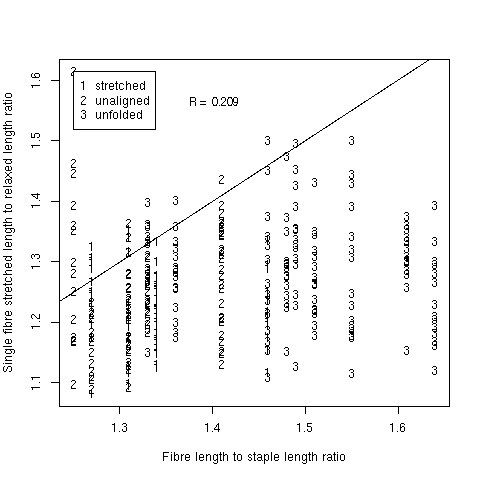
\includegraphics[width=1.1\textwidth]{figfibrelftolslftolr.png}
% original is  15fibrepredLftoLrmedian.png
  \caption{Plot of measured fibre stretched length to relaxed length ratio for 15 fibres per sheep, against measured mean fibre stretched length to staple length ratio for each sheep. }
  \label{fig:fibrelftolslftolr}
\end{figure}

%\end{document}

